\documentclass{standalone}

\usepackage{tikz}
\usepackage{bm}
\usepackage{amsmath}
\usetikzlibrary{calc, tikzmark, shapes, shapes.arrows, arrows, positioning}
\newcommand{\mat}[1]{\boldsymbol{\rm{#1}}}
\newcommand{\T}{\mat{T}}
\renewcommand{\vec}[1]{\boldsymbol{#1}}

\begin{document}
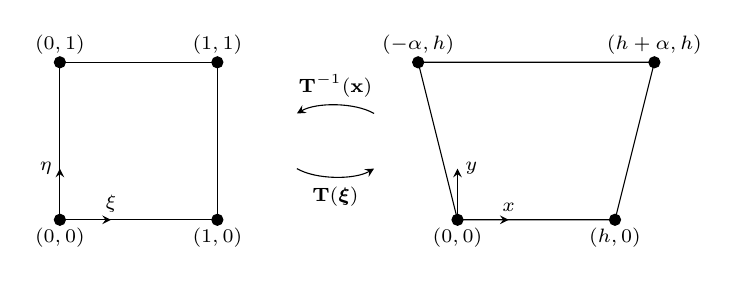
\begin{tikzpicture}
\scriptsize
\begin{scope}[xshift=-2.5cm]
	\filldraw[black] (-1,-1) circle[radius=2pt] node[below] {$(0,0)$};
	\draw[->, >=stealth] (-1,-1) -- (-.35,-1) node[above] {$\xi$}; 
	\draw[->, >=stealth] (-1,-1) -- (-1,-.35) node[left] {$\eta$}; 
	\filldraw[black] (1,-1) circle[radius=2pt] node[below] {$(1,0)$};
	\filldraw[black] (-1,1) circle[radius=2pt] node[above] {$(0,1)$};
	\filldraw[black] (1,1) circle[radius=2pt] node[above] {$(1,1)$};
	\draw (-1,-1) -- (1,-1) -- (1,1) -- (-1,1) -- (-1,-1); 
\end{scope}
\draw[->, >=stealth, shorten >= 3mm, shorten <= 3mm] (-.75,-.2) to [bend right=30] (.75,-.2); 
\node at (0,-.7) {$\T(\vec{\xi})$}; 
\draw[->, >=stealth, shorten >= 3mm, shorten <= 3mm] (.75,.2) to [bend right=30] (-.75,.2); 
\node at (0,.7) {$\T^{-1}(\mat{x})$}; 
\begin{scope}[xshift=2.55cm]
	\filldraw[black] (-1,-1) circle[radius=2pt] node[below] {$(0,0)$};
	\draw[->, >=stealth] (-1,-1) -- (-.35,-1) node[above] {$x$}; 
	\draw[->, >=stealth] (-1,-1) -- (-1,-.35) node[right] {$y$}; 
	\filldraw[black] (1,-1) circle[radius=2pt] node[below] {$(h,0)$};
	\filldraw[black] (-1.5,1) circle[radius=2pt] node[above] {$(-\alpha,h)$};
	\filldraw[black] (1.5,1) circle[radius=2pt] node[above] {$(h+\alpha,h)$};
	\draw (-1,-1) -- (1,-1) -- (1.5,1) -- (-1.5,1) -- (-1,-1); 
\end{scope}
\end{tikzpicture}
\end{document}